\section{Riktantenner för kortvåg}

\subsection{Riktbar dipol-antenn}

\begin{figure}
  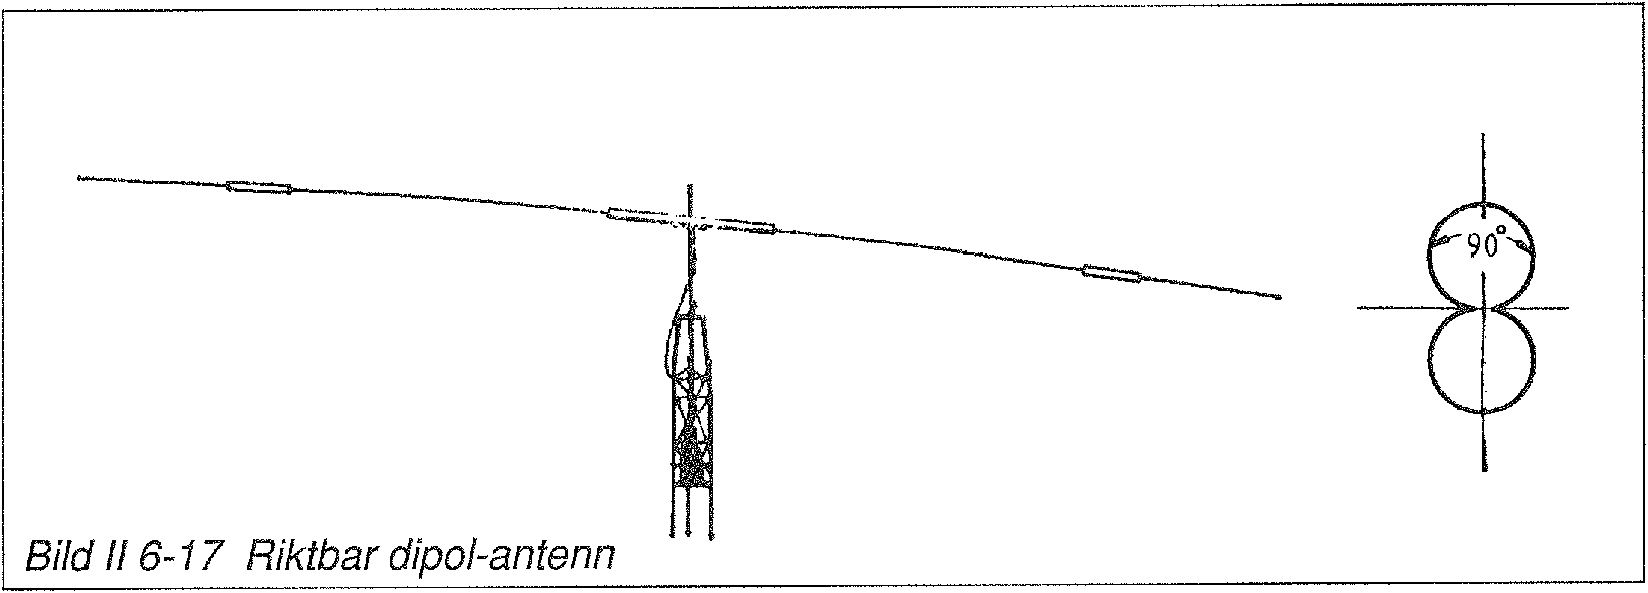
\includegraphics[width=\textwidth]{images/bild_2_6-17}
  \caption{Riktbar dipol-antenn}
  \label{fig:bildII6-17}
\end{figure}

Bild \ref{fig:bildII6-17}

En dipolantenn av måttlig mekanisk storlek kan göras vridbar så att
utstrålningen kan riktas. Men eftersom en ensam dipol strålar i många
riktningar, låtvara mest vinkelrätt ut från antennen, så är energin i
flesta riktningarna att ses som ``förlorad''. När ett passivt
antennelement - en reflektor - placeras bakom det aktiva elementet kan
emellertid bakåtstrålningen delvis vändas framåt och man får i stället
en viss riktverkan. För att det ska fungera ska de båda elementen
ha en viss inbördes längd och ett visst avstånd emellan.


\subsection{Yagi-antenner}
\textbf{
HAREC a.\ref{HAREC.a.6.1.5}\label{myHAREC.a.6.1.5}
}

\begin{figure}
  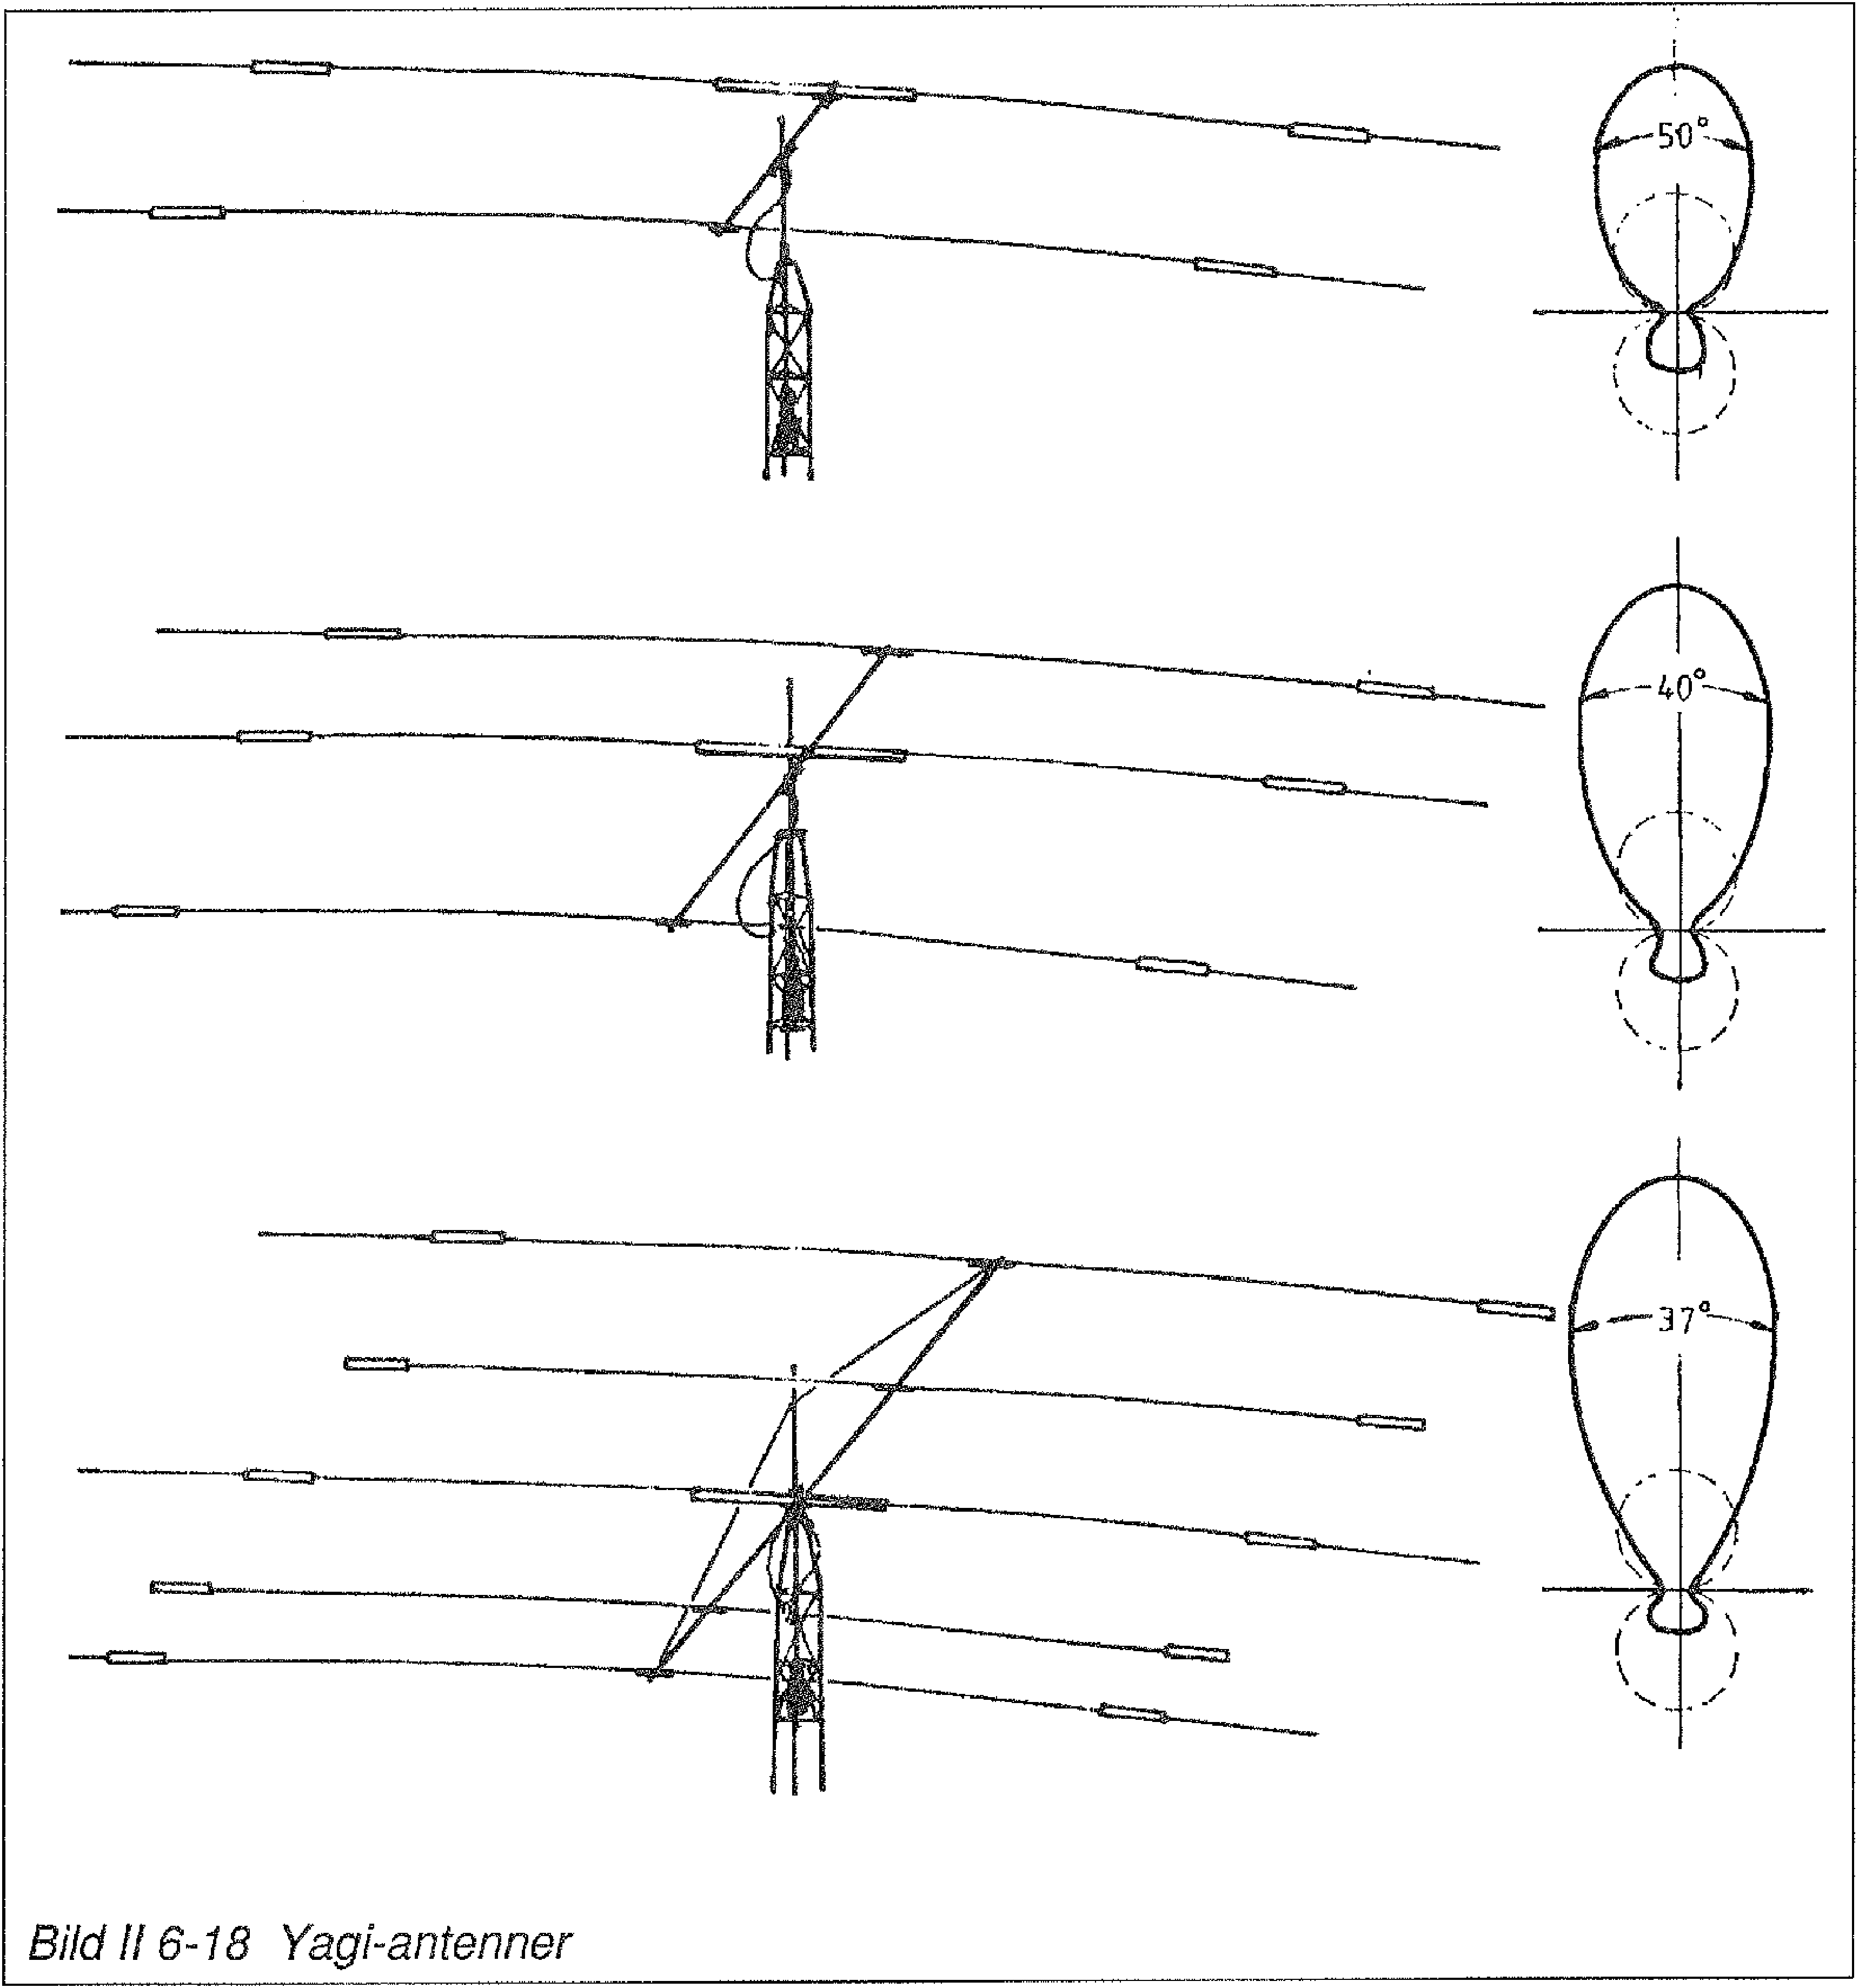
\includegraphics[width=\textwidth]{images/bild_2_6-18}
  \caption{Yagi-antenner}
  \label{fig:bildII6-18}
\end{figure}

Bild \ref{fig:bildII6-18}

Med ytterligare passiva antennelement - s.k. direktorer - framför det
aktiva elementet, blir riktverkan ännu bättre. Reflektorn är alltid
elektriskt längre än strålaren och direktorerna alltid elektriskt
kortare och allt kortare ju längre bort från strålaren. En sådan
antenn kallas Yagi-antenn, efter sin japanske upphovsman. Den är
ursprungligen avsedd för ett enda frekvensband, en s.k. monobandbeam.

Om alla element förses med lämpliga spärrkretsar, med W3DZZ-antennen
som förebild, fås en riktantenn som är användbar på flera
frekvensband, en s.k. multibandbeam. De vanligaste flerbandsantennerna
är konstruerade för 20 m-, 15 m- och 10 m-banden och har två till tre
element.  Bilden visar riktbara multibandantenner med 2, 3 resp 5
element samt deras strålningsdiagram i horisontalplanet.  Matningen
sker oftast med en koaxialkabel med 50 Ω karakteristisk
impedans. Eftersom matningsimpedansen för själva riktantenn nästan
aldrig är 50 Ω, så behövs oftast en impedansanpassning mellan antenn
och kabel.

\subsection{Cubical Quad-antenner}

\begin{figure}
  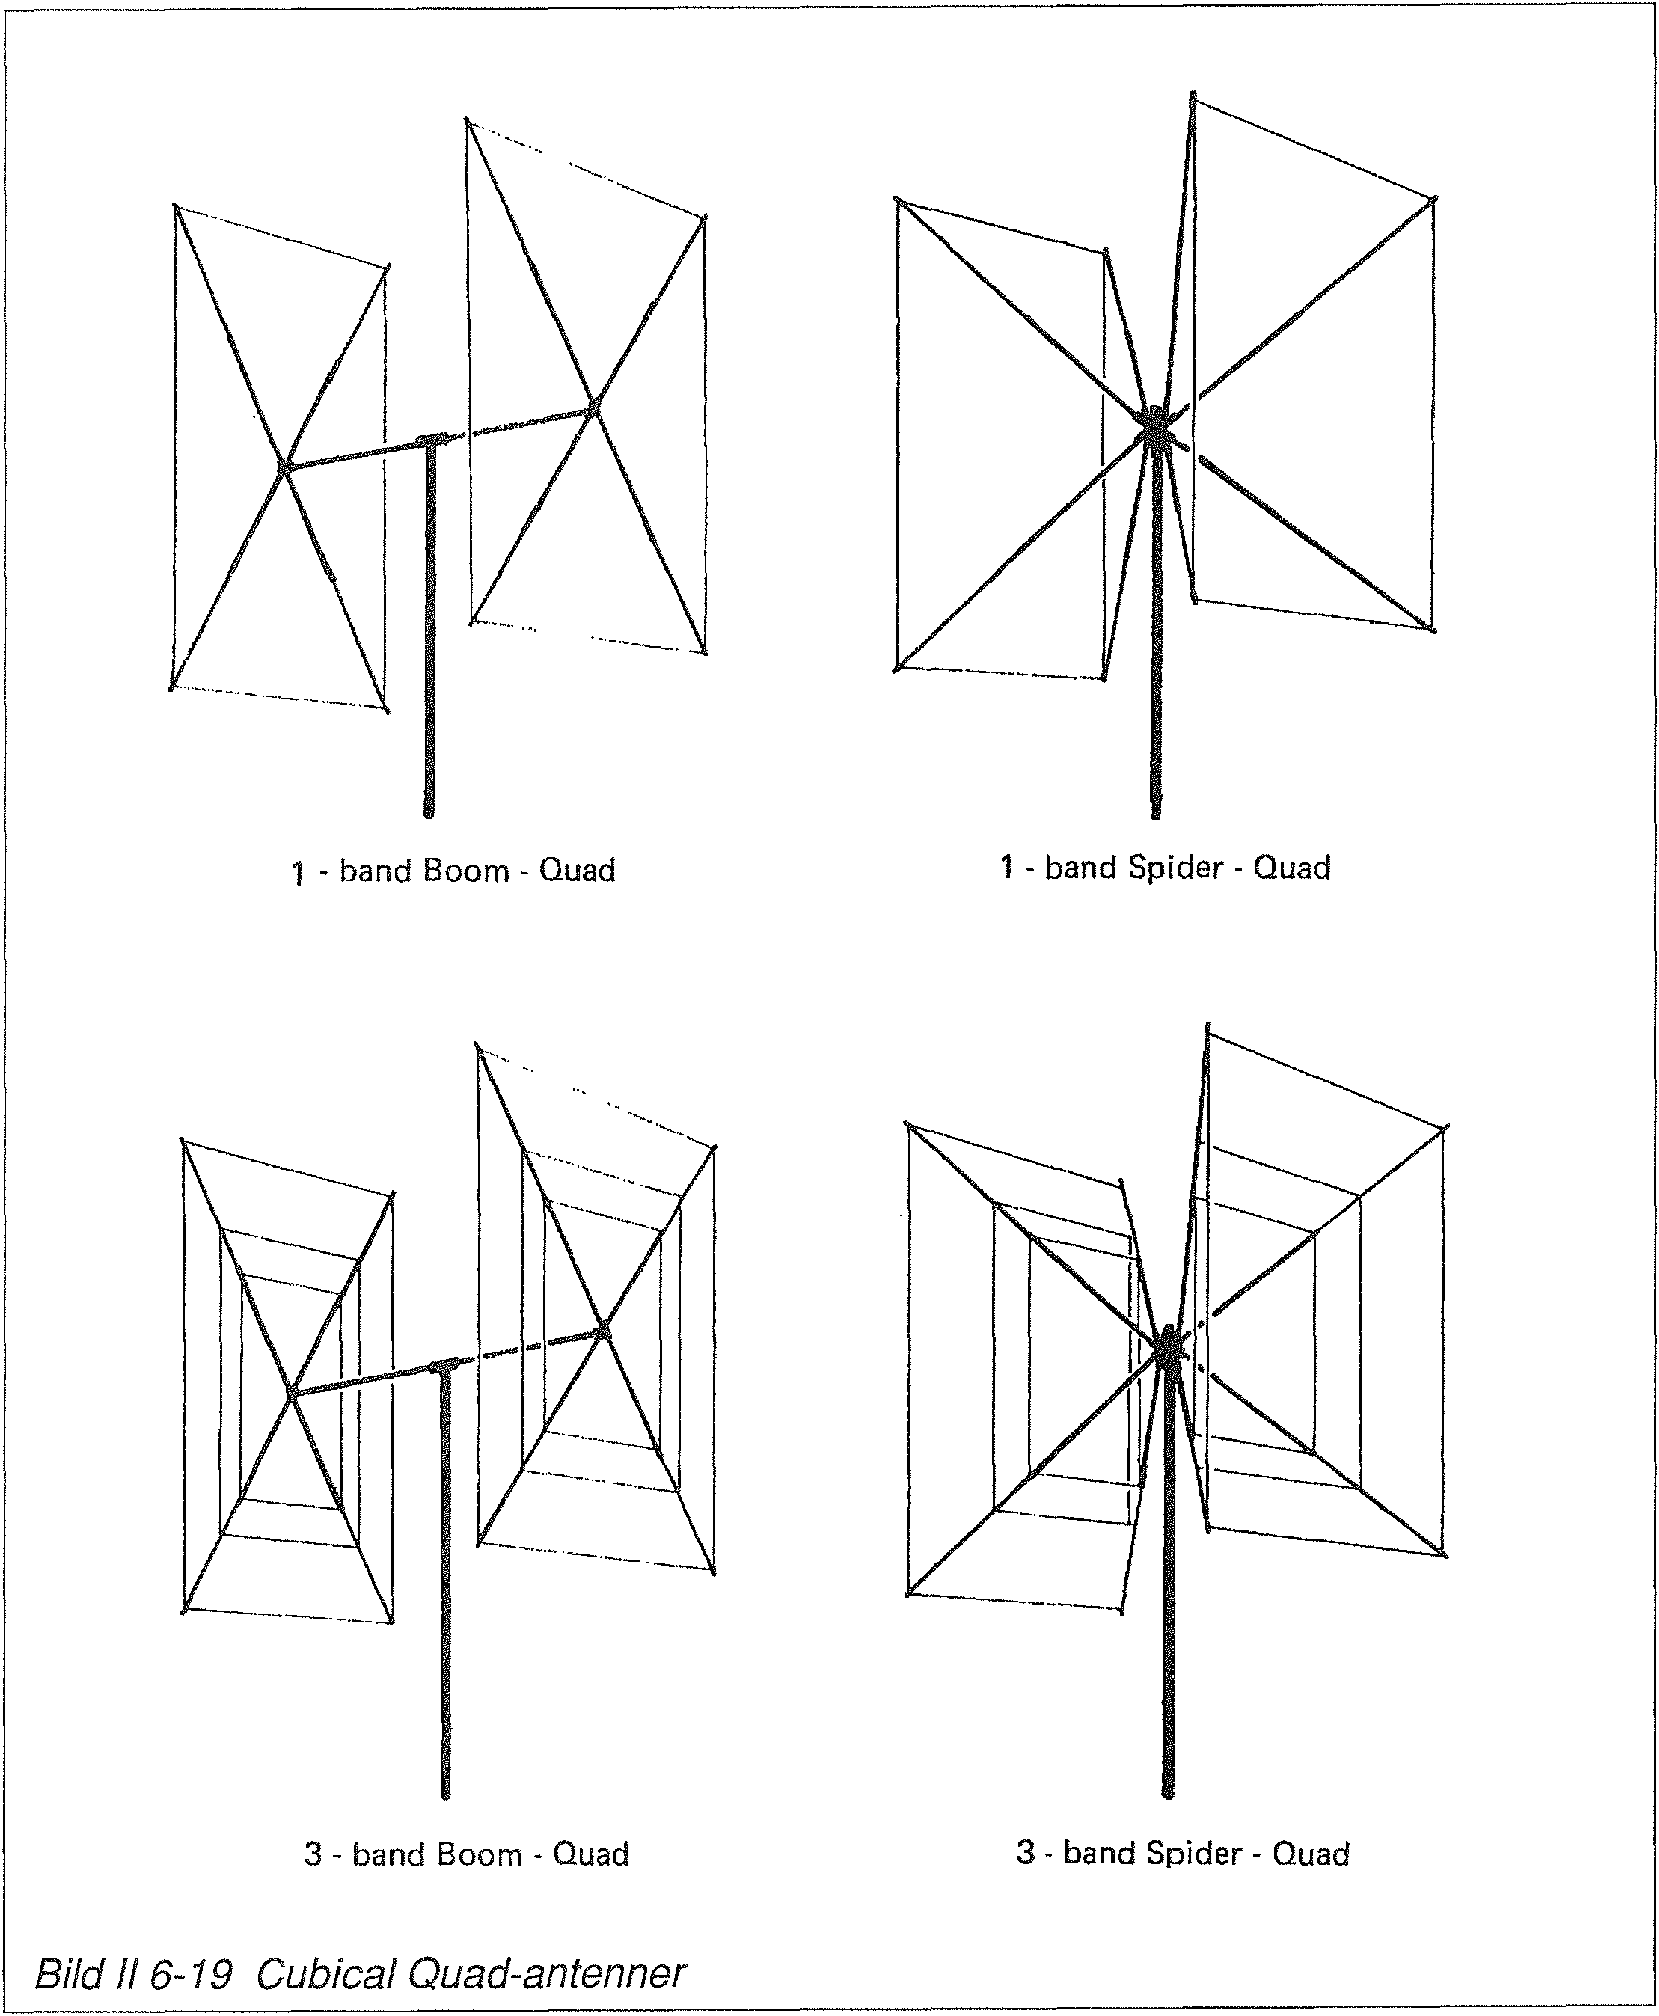
\includegraphics[width=\textwidth]{images/bild_2_6-19}
  \caption{Cubical Quad-antenner}
  \label{fig:bildII6-19}
\end{figure}

Bild \ref{fig:bildII6-19}

Cubical quad-antennen är en kvadratisk helvågsstrålare med en sidlängd
av \(\lambda/4\), d.v.s. totalt \(1\lambda\).

En 2-elements quad-antenn består av en strålare och en reflektor på
ett inbördes avstånd av 0,15 - 0,2 \(\lambda\). Det finns även 3 och
4-elements quad-konstruktioner med beaktansvärda dimensioner. Antennen
görs lämpligen vridbar och bör monteras åtminstone \(3/4 \lambda\)
över mark.

Matningsimpedansen är 50 - 70 Ω, beroende på elementavståndet.
Matningen sker oftast med en koaxialkabel. Beroende på hur
matningspunkten placeras är det möjligt att välja mellan kan
horisontell eller vertikal polarisering.

Det finns två utföranden av quad-antenner, det ena med en bärande bom
med spridare för att bära upp antennelementen och det andra med bara
spridare från ett centralt fäste, den s.k. spider quad (spindel).

Quad-antennen byggs för vanligen för 20 m-, 15 m- och 10
m-banden. Spiderprincipen är att föredra vid flerbandsutförande,
eftersom ett optimalt elementavstånd kan väljas för varje band utan
att spridarantalet behöver ökas.

Genom den flacka strålningsvinkeln är quad-antennen en utmärkt
DX-antenn. En två-elements quad anses kunna ge ett resultat som en
3-elements Yagi-antenn.

För kortvågsbruk finns många antenntyper, såsom longwire-, zepp-,
windom-, romb-, delta loop-, quad loop-antenner etc. För mer
information hänvisas till antennlitteratur.
